\documentclass[a4paper,10pt,DIV=14]{article}
\usepackage{graphicx}
\usepackage[utf8]{inputenc} % korrekte Darstellung von Umlauten u. Sonderzeichen
\usepackage[ngerman]{babel} % Sprachpaket, ngerman = neue deutsche Rechtschreibung
\usepackage{amsmath} % Setzen mathematischer Formeln
\usepackage{amsfonts} %mathbb
\usepackage{titlesec}
\usepackage{float}
\usepackage{caption}
\usepackage{fancyvrb}
\usepackage{siunitx}
\usepackage{booktabs}
\usepackage{enumitem}
\usepackage{tikz}

\usepackage{tabularx}
\newcolumntype{L}[1]{>{\raggedright\arraybackslash}p{#1}} % linksbündig mit Breitenangabe
\newcolumntype{C}[1]{>{\centering\arraybackslash}p{#1}} % zentriert mit Breitenangabe
\newcolumntype{R}[1]{>{\raggedleft\arraybackslash}p{#1}} % rechtsbündig mit Breitenangabe

\newcommand{\gqq}[1]{\glqq{}#1\grqq{}}
\newcommand{\gq}[1]{\glq{}#1\grq{}}
\newcommand{\dg}[1]{#1^\circ}

\renewcommand{\thesection}{Aufgabe \arabic{section}:}
\renewcommand{\thesubsection}{\alph{subsection})}
\renewcommand{\thesubsubsection}{\roman{subsubsection}}

\titleformat{\subsection}
{\normalsize}{\thesubsection}{1em}{}


\captionsetup[figure]{labelformat=empty}

\begin{document}

\title{Graphische Datenverarbeitung WS17/18 \\ Theorieübung 3}
\author{
  Salmah Ahmad (2880011)
  \and
  Markus Höhn (1683303)
  \and
  Tobias Mertz (2274355)
  \and
  Steven Lamarr Reynolds (1620638)
  \and
  Sascha Zenglein (2487032)
}

\maketitle

\section{Räumliche Datenstrukturen (2 Punkte)}

\subsection{(1 Punkt)}
BSP-Baum:\\
\begin{tikzpicture}[sibling distance=5cm, level distance=1.8cm,
level 1/.style={sibling distance=3cm},
level 2/.style={sibling distance=1.5cm},  
  every node/.style = {shape=circle, rounded corners,
    draw, align=center,
%    top color=white, bottom color=blue!20
	}]]
  \node[minimum size=1cm] {A}
    child[minimum size=1cm] { node {$B_1$} 
    	child[minimum size=1cm] { node {$C_1$}
    		child[minimum size=1cm] { node {E}}
    		child[missing, minimum size=1cm] {node {}}
    	}
    	child[minimum size=1cm] { node {F}}
    }
    child[minimum size=1cm] { node {G}
      child[minimum size=1cm] { node {H}}
      child[minimum size=1cm] { node {D}
			child[minimum size=1cm] { node {$C_2$}}     
			child[minimum size=1cm] { node {$B_2$}}
		}
      };
\end{tikzpicture}

\subsection{(1 Punkt)}
Zeichenreihenfolge (Zuerst $\rightarrow$ Zuletzt):\\
H, G, $B_2$, D, $C_2$, A, $C_1$, E, $B_1$, F

\section{Projektionen (5 Punkte)}

\subsection{a)}
\subsubsection{i}
$f_l= \begin{pmatrix}
tan(\frac{\theta}{2})\cdot f \\
f \\
\end{pmatrix}$ \\
$f_r= \begin{pmatrix}
-tan(\frac{\theta}{2})\cdot f \\
f \\
\end{pmatrix}$ \\
$n_l= \begin{pmatrix}
tan(\frac{\theta}{2})\cdot n \\
n \\
\end{pmatrix}$ \\
$n_r= \begin{pmatrix}
-tan(\frac{\theta}{2})\cdot n \\
n \\
\end{pmatrix}$ 

\subsubsection{ii}

\begin{figure}[!htbp]
	\centering
	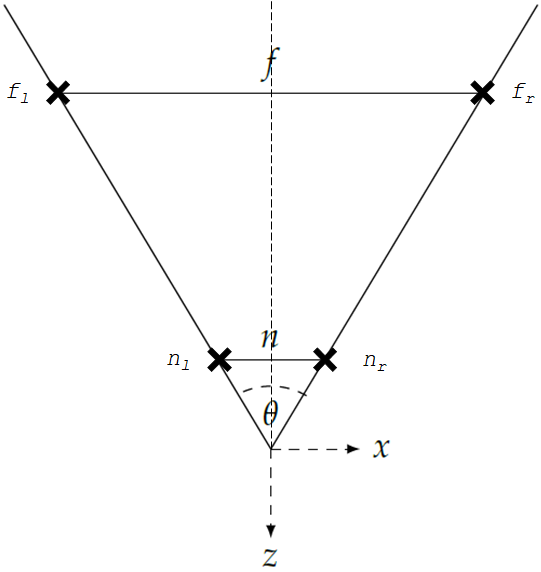
\includegraphics[width=1\linewidth]{frustum}
\end{figure}

$f_l= 
\begin{pmatrix}
	1 & 0 & 0  \\
	0 & 1+\frac{-f}{-n} & -f  \\
	0 & -\frac{1}{-n} & 0  \\
\end{pmatrix} \cdot
\begin{pmatrix}
	tan(\frac{\theta}{2})\cdot f \\
	f \\
	1 \\
\end{pmatrix}
= 
\begin{pmatrix}
	-\frac{-n}{f} \cdot tan(\frac{\theta}{2})\cdot f\\
	-\frac{-n}{f} \cdot(-f)-(-f-n) \\
	1 \\
\end{pmatrix}\\
= 
\begin{pmatrix}
	n \cdot tan(\frac{\theta}{2})\\
	f \\
	1 \\
\end{pmatrix}
$ \\
$f_r= 
\begin{pmatrix}
	1 & 0 & 0  \\
	0 & 1+\frac{-f}{-n} & -f  \\
	0 & -\frac{1}{-n} & 0  \\
\end{pmatrix} \cdot
\begin{pmatrix}
	-tan(\frac{\theta}{2})\cdot f \\
	f \\
	1 \\
\end{pmatrix}
=
\begin{pmatrix}
	-\frac{-n}{f} \cdot(-tan(\frac{\theta}{2}))\cdot f\\
	-\frac{-n}{f} \cdot(-f)-(-f-n) \\
	1 \\
\end{pmatrix}\\
= 
\begin{pmatrix}
	-n \cdot tan(\frac{\theta}{2})\\
	f \\
	1 \\
\end{pmatrix}
$ \\
$n_l= 
\begin{pmatrix}
	1 & 0 & 0  \\
	0 & 1+\frac{-f}{-n} & -f  \\
	0 & -\frac{1}{-n} & 0  \\
\end{pmatrix} \cdot
\begin{pmatrix}
	tan(\frac{\theta}{2})\cdot n \\
	n \\
	1 \\
\end{pmatrix}
=
\begin{pmatrix}
	-\frac{-n}{n} \cdot tan(\frac{\theta}{2})\cdot n\\
	-\frac{-n}{n} \cdot(-f)-(-f-n) \\
	1 \\
\end{pmatrix}\\
= 
\begin{pmatrix}
	n\cdot tan(\frac{\theta}{2})\\
	n \\
	1 \\
\end{pmatrix}
$ \\
$n_r= 
\begin{pmatrix}
	1 & 0 & 0  \\
	0 & 1+\frac{-f}{-n} & -f  \\
	0 & -\frac{1}{-n} & 0  \\
\end{pmatrix} \cdot
\begin{pmatrix}
	-tan(\frac{\theta}{2})\cdot n \\
	n \\
	1 \\
\end{pmatrix}
=
\begin{pmatrix}
	-\frac{-n}{n} \cdot(-tan(\frac{\theta}{2}))\cdot n\\
	-\frac{-n}{n} \cdot(-f)-(-f-n) \\
	1 \\
\end{pmatrix}\\
= 
\begin{pmatrix}
	-n \cdot tan(\frac{\theta}{2})\\
	n \\
	1 \\
\end{pmatrix}
$ \\

\subsubsection{iii}
$r = n \cdot tan(\frac{\theta}{2}) \qquad  l = -n \cdot tan(\frac{\theta}{2})
$\\
$f'_l=
P_0 \cdot f_l =
\begin{pmatrix}
    \frac{2}{r-l} & 0 & \frac{r+l}{l-r}\\
    0 & \frac{2}{f-n} & \frac{-f-n}{f-n}\\
    0 & 0 & 1\\
\end{pmatrix} \cdot
\begin{pmatrix}
    n \cdot tan(\frac{\theta}{2})\\
    f\\
    1\\
\end{pmatrix}$\\$ = 
\begin{pmatrix}
    \frac{1}{n \cdot tan(\frac{\theta}{2})} & 0 & 0\\
    0 & \frac{2}{f-n} & \frac{-f-n}{f-n}\\
    0 & 0 & 1\\
\end{pmatrix} \cdot
\begin{pmatrix}
    n \cdot tan(\frac{\theta}{2})\\
    f\\
    1
\end{pmatrix} =
\begin{pmatrix}
    1\\
    1\\
    1\\
\end{pmatrix}
$\\
$f'_r=
P_0 \cdot f_r =
\begin{pmatrix}
    \frac{1}{n \cdot tan(\frac{\theta}{2})} & 0 & 0\\
    0 & \frac{2}{f-n} & \frac{-f-n}{f-n}\\
    0 & 0 & 1\\
\end{pmatrix} \cdot
\begin{pmatrix}
    -n \cdot tan(\frac{\theta}{2})\\
    f\\
    1
\end{pmatrix} =
\begin{pmatrix}
    -1\\
    1\\
    1\\
\end{pmatrix}
$\\
$n'_l=
P_0 \cdot n_l =
\begin{pmatrix}
    \frac{1}{n \cdot tan(\frac{\theta}{2})} & 0 & 0\\
    0 & \frac{2}{f-n} & \frac{-f-n}{f-n}\\
    0 & 0 & 1\\
\end{pmatrix} \cdot
\begin{pmatrix}
    n \cdot tan(\frac{\theta}{2})\\
    n\\
    1
\end{pmatrix} =
\begin{pmatrix}
    1\\
    -1\\
    1\\
\end{pmatrix}
$\\
$n'_r=
P_0 \cdot n_r =
\begin{pmatrix}
    \frac{1}{n \cdot tan(\frac{\theta}{2})} & 0 & 0\\
    0 & \frac{2}{f-n} & \frac{-f-n}{f-n}\\
    0 & 0 & 1\\
\end{pmatrix} \cdot
\begin{pmatrix}
    -n \cdot tan(\frac{\theta}{2})\\
    n\\
    1
\end{pmatrix} =
\begin{pmatrix}
    -1\\
    -1\\
    1\\
\end{pmatrix}$\\

\subsection{b)}
\subsection{c)}
\subsection{d)}

\section{Clipping (3 Punkt)}

\end{document}
